% -*-mode: Latex-*-
% !TEX root = thesis.tex
% paper: ...
% authors: simon maurer
%
% file: background.tex
% contents: background of the thesis
% Sccs-Id: %W% %G%
\chapter{Background}
\label{chap_background}

In this chapter I will discuss terminology and give some background on topics relevant for this dissertation.
% This includes an introduction into \gls{cps} and the challenges software engineers are facing when developing \gls{cps}, a short survey on coordination languages and their history as well as work that relates coordination languages to \gls{cps}.

The chapter is structured as follows:
\Sect{\ref{sect_background_term}} discusses the term \emph{real-time} and its ambiguous meaning in different research areas and relates embedded systems to \glspl{cps} and \gls{iot}.
\Sect{\ref{sect_background_comp}} describes the basic idea of component-based design, the approach used as a corner stone for the \gls{pnsc} model proposed in this dissertation.
I then describe properties of \glspl{cps} and discuss their relevance with respect to the design approach of \glspl{cps} in \Sect{\ref{sect_background_cps}}.
\Sect{\ref{sect_background_com}} focuses on communication aspects such as the triggering semantics, \ie time-triggered or event-triggered communication and communication coupling.
\Sect{\ref{sect_background_coord}} provides a short history on coordination languages and discusses classification aspects of coordination languages.

%==============================================================================
\section{A Side-note on Terminology}
\label{sect_background_term}
Traditionally, a hard real-time system describes a system where the consequence of missing a deadline may result in a catastrophic event.
Hence, the correctness criteria of a piece of software not only rely on the correctness of the result but also on the time of availability of the result.
If the software provides a correct result but misses the deadline by doing so, the correctness criteria are not met.
One tends to distinguish between hard real-time systems and soft real-time systems where the latter also imposes a deadline but the consequences of missing a soft deadline are less severe.
By missing a soft deadline, the quality of the result only decreases but does not become useless.

There are two general points I want to make concerning the concepts of real-time systems.
Firstly, I find that the distinction between best effort systems and soft real-time systems is only marginal and that a soft real-time system has much more in common with a best-effort application than with a hard real-time system.
Ultimately, every system has a soft deadline because if a computation is never producing a result, the computation is hardly useful.
Hence, technically, every system is a real-time system.
However, there is a difference in terms of the usefulness of a result depending on when it is available.
In the case of a best effort application, the expectation is that eventually a result will be available (before a non-specified deadline $< \infty$) and the sooner it is available the better.
With soft real-time systems, the expectation is put into numbers, meaning that the application is expected to deliver a result within a specified deadline and there is no immediate benefit if the result is available earlier.
In contrast to a hard real-time system where the focus lies on giving \emph{guarantees} to meet deadlines, in soft real-time systems no guarantees are given that a deadline is met.
Rather, methods are used to decrease the possibility for deadlines to be missed.
For example, in the case of a video stream application, buffers are used to store frames that resulted before the deadline in order to compensate during times when the deadline is missed.

The second point concerns the use of the term \emph{real-time} which has an ambiguous meaning depending on the research community.
Most commonly, in research, the term real-time describes the fact that an application has to respect a deadline, \ie a result must be made available before a specified time limit has passed.
However, I found that a lot of people, not necessarily researchers, associate the term real-time with simultaneously performing a computation as a direct reaction on events happening in the world, \eg a football live stream, the logging of events while they are happening, the capturing and visualising of human motions while the human is performing the motions, etc.
All these problems are probably designed and programmed, using in one way or another the notion of a deadline but the term real-time does not reflect that.
Rather it reflects liveness of an application which creates, in my opinion, unnecessary confusion when explaining such problems to non-experts.
Following the argument I made above that soft real-time and best-effort applications are more closely related than hard real-time problems are related to soft real-time problems, I advocate to use the term \emph{time-critical} when talking about hard real-time problems.
It immediately carries the message that time plays a critical part in such an application and avoids the confusion with live systems.
Hence, throughout this dissertation I will use the term \emph{time-critical} system when talking about a hard real-time system.

Time-critical systems are tightly coupled to the hardware they are running on.
This is because the execution time of an application is dependent on the hardware architecture and to give guarantees that an application will meet the specified deadlines, it is important to fully understand the associated hardware architecture.
Due to this, in the past, target hardware platforms for time-critical systems were often specialised boards fulfilling the exact requirements to provide the resource demands of the software application executed on the platform.
As components on such boards were directly soldered on, such hardware boards were called \emph{embedded systems} and the term became synonymous for \emph{hard real-time systems} (or time-critical systems as I call them), including software and hardware components.
With the evolution of hardware architectures, computational units were and still are becoming increasingly efficient and performant.
Combined with the increasing demand for smarter, time-critical applications it often became necessary to build networked systems where not one single platform was used.
Also, a lot of devices of today are embedded on a single board without necessarily hosting a time-critical system.
Literally, the term \emph{embedded system} only describes the technique of how a hardware board is assembled which is no longer an indication that the executed application is actually a time-critical system.
Despite the potential confusion, the term \emph{embedded system} is still used to describe a single platform, time-critical system.
However, more complex systems, including multiple networked time-critical platforms, \ie embedded systems, are referred to as \emph{\acrfullpl{cps}}.
The focus of the term \gls{cps} is put on the interaction between the physical and the cyber world through sensors and actuators.

Another term that relates to similar concepts is \emph{\acrfull{iot}}.
An \gls{iot} is an instance of the more general term \gls{cps}.
It describes largely distributed applications where each "thing" represents a node in a network of interacting nodes.

Note that neither embedded systems, nor \glspl{cps}, nor the \gls{iot} must necessarily describe time-critical applications but as they interact with the physical world they generally do have timing constraints.

%==================================================================
\section{Component-based Design}
\label{sect_background_comp}
Component-based design aims at separating concerns by dividing large systems into loosely coupled independent, concurrent components~\cite{deAlfaro2005, gossler2002}.
This concept is a corner stone of a multitude of models, for example, in the area of stream processing~\cite{stephens1997} or coordination languages~\cite{papadopoulos1998}.
Typically, these models describe a composition of computational components that form a network.
Linking structures, such as channels or shared memory locations, establishes connections between components.
Such networks are usually explicitly constructed with the help of either a language (\eg StreamIt~\cite{thies2002} or S-Net~\cite{grelck2010} where networks are constructed by applying binary wiring operators on components) or a library (\eg Open MPI~\cite{open-mpi} which provides an API to spawn channels linking components together).
The question of compatibility between components is either inherently solved by construction of the language (S-Net only allows functional components and uses component signatures to check for compatibility) or is delegated to the programmer (Open MPI).

In component-based design, implementation details of components are often ignored and a component is represented by an abstraction.
The key is to choose an abstraction that allows to describe the component accurately enough to expose certain properties while keeping the abstraction as simple as possible~\cite{deAlfaro2005}.
By composing simple components to build complexer ones, the properties exposed by the abstraction are used to check for compatibility of the components.
Ideally, such a model supports heterogeneous systems and unifies the compatibility problem within one model~\cite{gossler2002}.
In order for the programmer to be able to cope with concurrent systems, models have been proposed to check interoperability of components either by using an automata-based interface description of components such as \glspl{ia}~\cite{deAlfaro2001a}, causality interfaces~\cite{zhou2006}, or transfer functions~\cite{thiele2006}, to name only a few.

A specific aspect of compatibility of components is the liveness property of a system composed of components.
A system is not guaranteed to be alive if a subset of the complete system or a subset of involved components can permanently block.
A widely known case of permanent blocking is a deadlock situation~\cite{coffman1971}.

In this dissertation I am interested in an automata-based approach to describe interfaces of components and use it to check for freedom of permanent blocking in the system.
My approach is inspired by \glspl{ia} but uses a different blocking semantics to make it suitable in the context of stream processing.


%==============================================================================
\section{Permanent Blocking and Deadlocks}
\label{sect_background_block}

In this dissertation I use the term \emph{liveness} to describe whether a system is void of any blocking subsystems.
I use the term \emph{permanent blocking} as the opposite of \emph{liveness}, \ie to describe a system that has at least one blocking subsystem:
\begin{equation}
    \label{eq_liveness}
    permanent\_blocking = \neg (liveness)
\end{equation}
Permanent blocking must not necessarily be a deadlock.
Coffman \etal identified four conditions that must hold simultaneously for a deadlock to occur~\cite{coffman1971}.
These conditions are listed in \Def{\ref{def_dl}}.

\begin{definition}[Four Deadlock Conditions]
    \label{def_dl}
    A system is in a deadlock situation if the following four conditions hold simultaneously:
    \begin{enumerate}
        \item \emph{Mutual exclusion:} a task has exclusive control over a resource.\label{enum_mutex}
        \item \emph{No pre-emption:} a resource can only be released voluntarily by the task holding it.\label{enum_preemption}
        \item \emph{Hold and wait:} a task is holding at least one resource and is requesting at least another.\label{enum_hold_wait}
        \item \emph{Circular wait:} a task $T_1$ is holding a resource $x$ and requests a resource $y$ while a task $T_2$ is holding resource $y$ and requests resource $x$.
            A circular wait is not necessarily limited to only two participants and can span over multiple parties.\label{enum_circular}
    \end{enumerate}
\end{definition}

A practical example of a deadlock, or more specifically a gridlock, is illustrated in Figure \ref{fig_cross_sync}.
It depicts an intersection of two roads where cars are assumed to only drive straight ahead without turning.
For a car, \eg arriving from the West, to be able to cross the intersection, two spaces, \eg $NW$ and $NE$, have to be allocated.
If traffic control allows to allocate spaces separately for cars arriving from each direction, the situation in Figure \ref{fig_cross_sync_b} can occur, where all spaces are occupied by an individual car such that no progression is possible for any car.
%------------------------------------------------------------------
\begin{figure}[bht]
    \TopFigSpace
    \centering
    \begin{subfigure}[t]{0.45\linewidth}
        \centering
        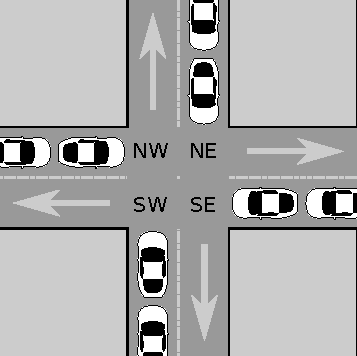
\includegraphics[width=5cm]{fig/cross_sync_a.pdf}
        \CaptionFigSpace
        \caption{A car has to allocate two spaces in order to advance.}
        \label{fig_cross_sync_a}
    \end{subfigure}
    ~
    \begin{subfigure}[t]{0.45\linewidth}
        \centering
        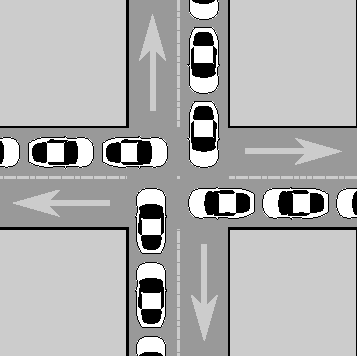
\includegraphics[width=5cm]{fig/cross_sync_b.pdf}
        \CaptionFigSpace
        \caption{A deadlock situation where no car is able to advance.}
        \label{fig_cross_sync_b}
    \end{subfigure}
    \caption{An example of gridlock on a crossing (no turning)}
    \label{fig_cross_sync}
    \BotFigSpace
\end{figure}
%------------------------------------------------------------------

It is possible that in a system of multiple interacting processes only one process is permanently blocked while the rest of the system is processing without permanently blocking.
If a process is blocking alone and no circular wait, as defined in \Def{\ref{def_dl}.\ref{enum_circular}}, is involved I call this process a \emph{lonely blocker}.
Hence, I distinguish between \emph{deadlock} where multiple components block each other due to a circular wait and \emph{lonely blocking} where one component is blocked by other components but is itself not causing other processes to block.

Therefore I conclude that
\begin{displaymath}
    permanent\_blocking \neq deadlock
\end{displaymath}
and consequently with \Equ{\ref{eq_liveness}} I conclude
\begin{displaymath}
    deadlock \neq \neg(liveness)
\end{displaymath}
However, deadlock implies permanent blocking, hence
\begin{displaymath}
    deadlock \rightarrow permanent\_blocking
\end{displaymath}
but permanent blocking does not necessarily imply deadlock:
\begin{displaymath}
    \neg(permanent\_blocking \rightarrow deadlock)
\end{displaymath}
Note that a permanent blocking process is either a lonely blocker or involved in a deadlock but not both.

Using again the example of a road intersection I illustrate a permanently blocking system that is not in a deadlock situation but rather a lonely blocking situation in \Fig{\ref{fig_cross_t}}.
%------------------------------------------------------------------
\begin{figure}[bht]
    \TopFigSpace
    \centering
    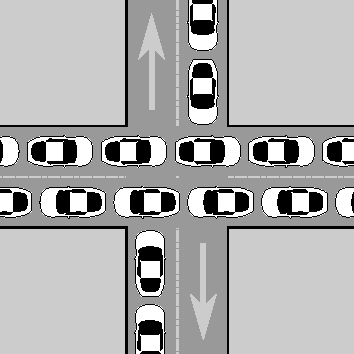
\includegraphics[width=5cm]{fig/cross_t.pdf}
    \CaptionFigSpace
    \caption{A lonely blocking situation where progress is only possible from the East to the West and vice versa.}
    \label{fig_cross_t}
    \BotFigSpace
\end{figure}
%------------------------------------------------------------------
While cars from the East are able to progress to the West and vice versa, cars in the North and in the South are blocked and cannot progress.
Assuming an infinite stream of cars and no priority rules, the cars from the North and the South will be blocked infinitely.
Note that this blocking is not due to a circular wait condition, as defined in \Def{\ref{def_dl}.\ref{enum_circular}}, because the cars moving from East to West and vice versa are not blocked.
Consequently, given that the system is in a permanent blocking situation without any deadlocks, the system is lonely blocking.

%==============================================================================
\section{Cyber-physical Systems}
\label{sect_background_cps}
\Glspl{cps} are systems that interact with the physical world through sensors and actuators.
Because the actuation is usually a reaction to the sensing of the environment, \glspl{cps} are generally \emph{reactive} and must often satisfy timing requirements.

Harel and Pnueli introduced the terms \emph{transformational} and \emph{reactive} to distinguish systems that are "relatively easy to develop from those that are not"~\cite{harel1985}.
In contrast to a transformational system that takes inputs, performs computation, and produces outputs, \glspl{cps} are often reactive systems where inputs are coupled to outputs via the environment.
The output $out$ of a transformational system, described by the function $f$, is dependent on the state $state$ of the system and the input $in$ to the system:
$$out = f(state,in)$$
Reactive systems, on the other hand, additionally, have a relation where the input $in$ of the system is not a variable but defined by a function $f_{env}$ which is dependent on the output of the system and an unknown variable $env$, imposed by the environment:
$$out = f(state,in) \ \land \ in = f_{env}(env,out)$$
Furthermore, a reactive system constantly reacts on changes in the environment while a transformational system is active on its own behalf.
These properties make it harder to decompose a reactive system in subcomponents which is less the case for transformational systems~\cite{harel1985}.
Kopetz distinguishes between \emph{simple} tasks (S-tasks) and \emph{complex} tasks (C-tasks)~\cite{kopetz2011a}.
A C-task contains blocking synchronisation points (\eg the task is blocking because it has to wait for the environment to provide it with an event) while an S-task does not.
A reactive system component tends to fit better with the C-task model and it can be hard to avoid this.
Consequently, reactive system components are often required to maintain a persistent state and to support bidirectional communication between components to allow an intuitive description of the reactive system.
While allowing persistent state in a system component makes it harder to exploit concurrency on parallel architectures, it has the benefit of making a model more accessible for legacy code.

The design and development of a \gls{cps} often involves a team of interdisciplinary experts to assemble the required knowledge to correctly model the interaction of the physical world with the cyber world.
As a consequence, different models from different application domains need to be brought together.
To cope with this Eker \etal~\cite{eker2003} proposed a unifying framework that allows to choose suitable models for each subsystem and assemble them through the framework.
More recent work proposes to focus on single meta-models with support for heterogeneity to increase the analysability of the model~\cite{henzinger2006, rajkumar2010, castrillon2015}.
The approach discussed in this dissertation aims towards this goal and is based on a component-based design approach (see \Sect{\ref{sect_background_comp}}).

To satisfy timing requirements of a \gls{cps}, the software components must be executed on a hardware platform that is able to provide the required resources.
For time-critical systems, guarantees must be provided that timing requirements are met, \ie such systems are designed for the worst case.
Guarantees are given by computing the \gls{wcet} of the software components, executed on a target platform.
Generally there are three different approaches to compute the \gls{wcet}:
By the conjunction of code analysis and a precise hardware model, by simulation, or by measurement through extensive testing.
The most commonly used technique in industry is the approach where extensive testing is performed in order to verify that requirements are satisfied~\cite{lee2008}.
The \gls{wcet} problem is nothing I will address in this dissertation but the interested reader might want to refer to the survey of Wilhelm \etal~\cite{wilhelm2008} for an overview of methods and available tools.

Another aspect of \glspl{cps} is \emph{mixed-criticality}.
With the increasing capability of hardware architectures, the need arises to execute multiple applications on the same hardware platform.
Often, there is a difference in terms of criticality of the applications intended for the same platform (\eg in a car, the multimedia system is of lower criticality than the parking assistance system).
In order to prevent interference from the low critical system to the high critical system, Vestal proposed a mixed-criticality scheduler~\cite{vestal2007}.
Burns and Davis provide an extensive review paper which they constantly update with new findings on the topic~\cite{burns2016}.
The focus of the research is almost exclusively on providing a scheduler, capable of scheduling a mixed-criticality application on single or multi-core architectures.
I am, however, interested in \gls{cci}, \ie an abstract model that allows components of different criticality levels to interact without interfering.

%==============================================================================
\section{Communication in Cyber-physical Systems}
\label{sect_background_com}
Human interaction with the physical world tends to be event-driven~\cite{tan2008}:
We react to sporadic changes in our environment and perform actions to adapt to the changes (turn the head upon registering a movement, keeping the balance on a ship).
The corresponding communication model for \glspl{cps} is the \emph{sporadic} or \emph{event-triggered} communication model.
In such a communication model, the transmission of information is triggered by the occurrence of events.
In a producer component, \ie a sensor, an event trigger occurs when a significant change of the state occurs which is then communicated to a consumer component.
The occurrence of events is sporadic, hence the time instant of the next event occurrence is unknown.
Due to this, it is hard to predict the required communication bandwidth and maximum load assumptions are needed in order to fulfil temporal constraints.
Local changes, like adding new components or changing the behaviour of an existing component, can invalidate the temporal behaviour of the system.
An event based communication scheme is useful for open systems and for systems with sporadic data.
Typical examples of deterministic models that are based on event-triggered communication are \glspl{kpn}~\cite{kahn1974} or the more restrictive \gls{sdf} model~\cite{lee1987}.

However, for critical applications where predictability and fault-tolerance are key, Kopetz \etal proposed the \gls{tta}~\cite{kopetz2011c}.
In a {\em time-triggered} communication scheme the participants use a common time basis and communicate at defined time instants.
The communication instants are often periodic due to simplicity but this is not a necessity.
Within a time-triggered communication system, local changes cannot invalidate the temporal behaviour of the system and the system load is independent of the number of message transmissions.
This is achieved through communication decoupling with temporal firewalls~\cite{kopetz2002}.
Due to the stability and predictability with respect to load and time behaviour, a time-triggered communication scheme is useful for fault tolerant systems.

Loosely coupled communication has also been studied in the domain of large distributed systems and three dimensions of coupling have been identified: time, space, and synchronisation (\cite{eugster2003, aldred2005}).
The three dimensions are orthogonal to each other.
In the following, a short description of each dimension is provided.

%------------------------------------------------------------------------------
\subsection{Communication Coupling in Time}
\label{sect_background_decoupling_time}
An interaction is time decoupled if the participating components are not required to operate at the same time in order to transmit messages.
In contrast, a time coupled interaction requires participants to operate at the same time for being able to communicate.
To achieve decoupling in time, a storage is necessary where messages can be placed by the sender until they are retrieved by the receiver.
Time decoupling allows the receiver to be disconnected at the time of the transmission by the sender and it allows the sender to be disconnected at the time of reception by the receiver.
The notion of time decoupling is binary.
Communication is either coupled or decoupled in time, there is no middle ground.

%------------------------------------------------------------------------------
\subsection{Communication Coupling in Space}
\label{sect_background_decoupling_space}
Communication is space decoupled if the involved parties do not know each other's address.
Contrary, in a space coupled interaction the sender uses a direct address of the receiver to transmit a message.
Space decoupling can be achieved by introducing an intermediate medium of communication.
This may be a shared storage, a channel for point-to-point communication, or a complex broker infrastructure taking care of the communication process.
Decoupling communication in space allows replacement and maintenance of components at runtime and is a prerequisite for open systems.

Decoupling in space is based on the notion of binding an address to a component.
If said address is known by the other communicating party the communication is coupled in space, otherwise, it is decoupled in space.
However, let's consider the example of a network component, addressed by its IP-address.
If this component is replaced with a new component using the exact same configuration, including the IP-address, the communication would work without any need for updating addresses in the participating communication parties.
Although, the recipient address must be known by the sender, this communication is space decoupled.
That is because the IP address is not an identification of the router (a MAC address would be tighter coupled but is still configurable) but a binding of an alias to a service.
It is not the component that the other communication parties are interested in, it is the service provided by that component (or any other component able to provide it).
Space decoupling is about the stability of an alias that is always providing an identical service, where the notion of identity means identical state and behaviour.

%------------------------------------------------------------------------------
\subsection{Communication Coupling in Synchronisation}
\label{sect_background_decoupling_sync}
Decoupling in synchronisation depends upon the read and write operation of the sender and receiver respectively.
Blocking operations imply a synchronous communication while non-blocking operations allow asynchronous transmission of messages.
To have a fully asynchronous interaction, both, writing and reading must be non-blocking.
Because coupling in synchronisation is an independent attribute of read and write operations, communication can be fully decoupled, partly decoupled or coupled in synchronisation.

In this dissertation the synchronisation decoupling is linked to forward and backward progress control.
Forward progress control describes the triggering semantics of the receiving component by a blocking read and backward progress control describes the back-pressure exert on the sending component by a blocking write.

%==============================================================================
\section{Coordination Languages}
\label{sect_background_coord}
The increasing system complexity of \glspl{cps} drives a high pressure on software engineering methodologies to assure an effective and predictable control of resources.
Coordination languages have been proposed as a solution to tackle this problem by decomposing application software into coordination and algorithmic programming~\cite{lee2008}.
The first coordination language, called \gls*{linda}, was introduced in 1992 by Gelrenter \etal~\cite{gelernter1992}.
The concept of \gls*{linda} is based on a shared memory space, called tuple space, where sets of data elements, called tuples, are placed and retrieved by processes with the help of specific primitives.
Over the years, several coordination languages, based on the tuple space paradigm, have been proposed~\cite{rossi2001, omicini2011}.
In their survey on coordination languages~\cite{papadopoulos1998}, Papadopoulos and Arbab distinguish between data-driven and control-driven coordination languages where \gls*{linda} and its derivates fall in the former class.
Data-driven coordination languages tend to provide some primitives that are used in the purely computational part to coordinate the exchange of information between processes.
This concept allows to build hierarchies and to broadcast information, two properties that are well suited for structured programming.
There is, however, not a strict separation between coordination and computation imposed by the model but the task of separating these concerns is left to the programmer.

Control-driven coordination languages, on the other hand, tend to enforce a clear separation of concerns because coordination elements are not part of the computational components.
This is usually achieved by linking computational components by channels or more complex coordination constructs~\cite{arbab1993, arbab2004}.
While data-driven models tend to coordinate data, control-driven models coordinate entities.
This model-based approach fits well with the world of \glspl{cps} where reactive components are common~\cite{henzinger2006, rajkumar2010, castrillon2015}.
A draw-back of the control-driven approach is that models often rely on point-to-point connections to describe the communication channels connecting computational components which lacks a clear structure.
However, Grelck \etal show with the coordination language \gls*{snet} that by using network operators, structured programming can also be achieved with a control-driven coordination model~\cite{grelck2010}.

Later, Arbab extended the classification of coordination languages and he introduced the terms \emph{endogenous} and \emph{exogenous} coordination, describing whether coordination is done from within a behavioural component or from the outside, respectively~\cite{arbab2006}.
An exogenous coordination model assures a clear separation between coordination and behaviour by leaving the behavioural components oblivious of the coordination constructs that exert coordination upon them.
An endogenous coordination model, on the other hand, has no such separation and the coordination is done from within a behavioural component which makes the component aware of the coordination exert on it.
A clear separation of concerns is important to simplify development, integration, and verification of applications.
In the domain of \glspl{cps} where systems are often safety critical, this is a property we need to enforce.

Lee suggested that the use of coordination models not only allows to separate behaviour and coordination but also provides an abstraction of the real-time behaviour from the underlying hardware platform~\cite{lee2008}.
An example of such an approach is the Ptides~\cite{derler2008} model (which is part of the Ptolemy project~\cite{ptolemaeus2014}) that allows to model timing behaviour of an event-triggered communication model.
Another example is Giotto which is a coordination language based on the time-triggered communication model~\cite{henzinger2001}.
With the concept of \gls{let}, Giotto provides a well defined input/output timing behaviour of interacting components that allow to loosen the coupling between the modelled timing specification and the timing behaviour of the application executed on a specific hardware platform.
